% TO-DO:
% * Actions = all possible transtions in RL
% * In RL, Q-learning is still unclear -- currently I'm using NN = transition F(x)
%   -- U(x) -> U(x') so it seems that generalization can occur in Q-space (?)
% * Structure of the turnstile is an important feature of the transition F(x)
% * Explain difference with AIXI
% * "inward" vs "outward"

\documentclass[orivec]{llncs}
\usepackage{graphicx}
\usepackage{amsmath}		% for "cases"
\usepackage{amsfonts}		% for frakur fonts
\usepackage{mathrsfs}		% for curly "E" error symbol
\usepackage{float}
\usepackage[most]{tcolorbox}% for wrapping example in color box
\usepackage{wrapfig}		% wrap figure beside text, used in example
\usepackage{tikz-cd}		% commutative diagrams
% \usepackage{amsfonts}
\usepackage[normalem]{ulem}	% underline with line breaks: /uline
\usepackage{enumitem}       % for using (A),(B),(C) in items...
\usepackage{amssymb}		% for \multimap, \updownarrow, \bigstar
\usepackage{turnstile}		% longer turnstiles
\usepackage{sectsty}		% change section color
\usepackage{hyperref}		% refs, links become clickable
\usepackage{url}			% for urls in bibliography
\usepackage[normalem]{ulem} % underline unbroken with \uline
\usepackage[numbers,sectionbib]{natbib}% if we use \package{url} we need to use natbib style

%\def\chinchin{yes}          % ********** 用中文 *********
% *************** Delete when not using Chinese or colors **********************
\ifdefined\chinchin
	\usepackage{xeCJK}
	\setCJKmainfont[BoldFont=SimHei,ItalicFont=KaiTi]{SimSun}
\fi
\usepackage{color}
%\newcommand{\emp}[1]{\textbf{\textcolor{blue}{#1}}}
\newcommand{\emp}[1]{\textbf{#1}}

\sectionfont{\color{blue}} 
\subsectionfont{\color{blue}} 
\subsubsectionfont{\color{blue}} 
\definecolor{green}{rgb}{0,0.7,0}
\definecolor{grey}{rgb}{0.95,0.95,0.95}

\usepackage{geometry}		% change paper size
\geometry{
  a4paper,         % or letterpaper
  textwidth=18cm,  % llncs has 12.2cm
  textheight=27cm, % llncs has 19.3cm
  heightrounded,   % integer number of lines
  hratio=1:1,      % horizontally centered
  vratio=2:3,      % not vertically centered
}
\usepackage[fontsize=13pt]{scrextend}

\newcommand{\tikzmark}[1]{\tikz[overlay,remember picture] \node (#1) {};}

\newcommand{\vect}[1]{\boldsymbol{#1}}
\newcommand*\sigmoid{\vcenter{\hbox{
\includegraphics{sigmoid.png}}}}
\newcommand*\rectifier{\vcenter{\hbox{\includegraphics{rectifier.png}}}}
\newcommand*\KB{\vcenter{\hbox{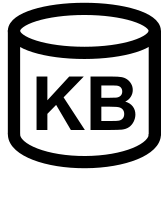
\includegraphics{KB-symbol.png}}}}
\newcommand*\KBsmall{\vcenter{\hbox{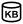
\includegraphics{KB-symbol2.png}}}}
\newcommand*\Eye{\vcenter{\hbox{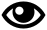
\includegraphics{../eye-symbol.png}}}}
\newcommand*\NN{\vcenter{\hbox{
\includegraphics{NN-symbol.png}}}}
\newcommand*\Graph{\vcenter{\hbox{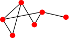
\includegraphics{algebraic-model.png}}}}
\newcommand{\dashh}{\textemdash~}
\newcommand{\english}[1]{\mbox{\textit{#1}}}
\newcommand{\tab}{\hspace*{2cm}}

% ***** Boxed variables inside math equations
% \newcommand*{\boxedcolor}{black}
\makeatletter
% \renewcommand{\boxed}[1]{\textcolor{\boxedcolor}{%
% \fbox{\normalcolor\m@th$\displaystyle#1$}}}
% \setlength{\fboxsep}{1pt}
\renewcommand{\boxed}[1]{\fbox{\m@th$\displaystyle\scalebox{0.9}{#1}$} \,}
\makeatother

\overfullrule=0mm

\newsavebox{\MyName}
\savebox{\MyName}{
\includegraphics[scale=0.6]{YKY.png}}

\ifdefined\chinchin
\title{神经网络中的「内省」\\
(``introspection'' in neural networks)}
\else
\title{``Introspection'' in neural networks}
\fi
%\normalsize{-- a minimalist cognitive architecture combining\\
%reinforcement learning and deep learning}}
\titlerunning{Introspection}
\author{\usebox{\MyName} (King-Yin Yan)
% \\ \footnotesize{General.Intelligence@Gmail.com}
%\and
%Ben Goertzel
%\and
%Juan Carlos Kuri Pinto
}
\institute{General.Intelligence@Gmail.com}
\date{\today}

\begin{document}
\let\labelitemi\labelitemii

\maketitle

\noindent
\makebox[\linewidth]{\small \today}

\setlength{\parindent}{0em}
\setlength{\parskip}{2.8ex plus0.8ex minus0.8ex}
% \setlength{\parskip}{2.8ex}

\begin{abstract}
在本文中「内省」是指智能系统直接读/写知识的能力,此能力在经典 logic-based AI 是免费做到的,但神经网络内的「知识」素来有「黑盒」的问题。  解决办法是让神经网络直接作用在它自身的 weights 上。  
\end{abstract}

%\begin{keywords}
%reinforcement learning, control theory, deep learning, cognitive architecture
%\end{keywords}

\setcounter{section}{-1}
\section{Introduction}
% \label{sec:0}

\ifdefined\chinchin
这篇文章说的「内省」的意思是指智能系统有能力读/写它内部的知识 \footnote{「内省」亦有 meta-reasoning 的意思,亦即除了\textbf{外在}的知识,系统还拥有关於系统自身状态的知识。 本文中「内省」是指存取「普通知识」的能力。}。  例如说,一个比较蠢的智能系统可以用 sequence-to-sequence 的方式将中文翻译成英文: 
\begin{equation}
\mbox{``}\boxed{中文句子}\mbox{''} \stackrel{\vect{F}}{\longrightarrow} \mbox{``}\boxed{英文句子}\mbox{''}
\end{equation}
$\vect{F}$ 代表系统的函数。  但系统并不真的明白句子的意义,句子只是「水过鸭背」地流过系统。 一个更聪明的系统是: 句子可以\textbf{进入}到 $\vect{F}$ 里。 我所说的「自省」就是这意思。
\else
By ``introspection'' is meant the ability of an intelligent agent to \textbf{access} (read or write) the contents of its knowledge base.  
\fi

Introspection is useful in:
\begin{itemize}
	\item learning by instructions, or ``learn by being told'' \\
	(a technique crucial to accelearating the learning of human knowledge)
	\item belief revision / truth maintenance \\
	(the most challenging and highest-level task in logic-based AI)
\end{itemize}

\ifdefined\chinchin
举例来说,小孩子的行为是由他内部的知识决定的,「知识决定行为」。
\begin{itemize}
	\item 当小孩子看到一个成人做的动作,他会模仿那动作。
	\begin{equation}
	\vcenter{\hbox{
\includegraphics[scale=0.5]{imitation.jpg}}}
	\end{equation}
	\item 或者小孩子听到一句说话:「不要吃污糟食物」,他明白了那句说话的意思而改变行为。
\end{itemize}
这两个例子都涉及到「感觉资料」进入 $\vect{F}$ 里面:
\begin{equation}
\boxed{sensory input} \hookrightarrow \vect{F}
\end{equation}
\else
For example, 
\fi

Introspection is related to the functional closure $\mathbb{X} \simeq \mathbb{X}^{\mathbb{X}}$ which gives a \textbf{Cartesian-closed category} (CCC).

\section{Architecture}

For reference, the architecture for \textbf{visual recognition} is:
\begin{equation}
\vcenter{\hbox{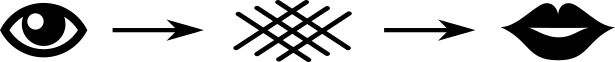
\includegraphics[scale=0.6]{vision-architecture.png}}}
\end{equation}
Our basic AGI architecture is:
\begin{equation}
\vcenter{\hbox{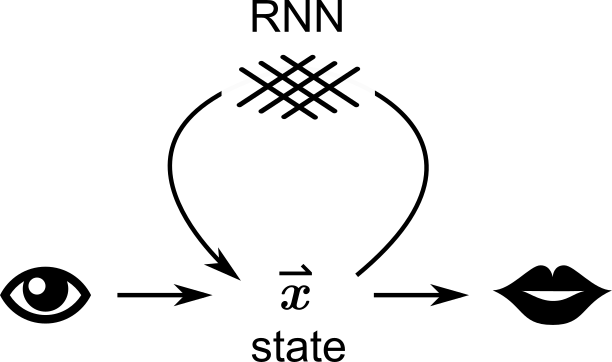
\includegraphics[scale=0.6]{basic-architecture.png}}}
\label{basic-arch}
\end{equation}

$\NN$ = [deep] neural network, trained via \textbf{reinforcement learning}

$\Graph$ = mental state / working memory

The main problems we need to solve for AGI:
\begin{enumerate}[label=(\Alph*)]
	\item How to enable a neural network to act on a graph structure (that does not easily fit into a fixed-length vector)?
	\item How to solve the introspection problem?
	\item How to incorporate \textbf{episodic memory} into the basic architecture (\ref{basic-arch})? \\
	Episodic memory may be essential for the learning of common-sense (eg. the need to process \textbf{stories}).
\end{enumerate}

We can use a deep network to emulate logical inference:
\begin{equation}
\NN \quad \Longleftrightarrow \quad \sststile{}{\KBsmall}
\end{equation}

$\sststile{}{\KBsmall}$ means to perform a \textbf{single step} of logical inference, ie, the \textbf{consequence operator}.

In the past, the learning of $\KB$ relied on \textbf{inductive logic learning}, based on combinatorial search, which was too slow.  The new hope is for deep learning to learn this mapping in reasonable time.

\ifdefined\chinchin
Deep learning 在 vision 中的成功,令我们相信它几乎可以 learn 出「任何 mapping」,除非那 mapping 具有 \uline{更深层} 的结构; 这时要用到 RNN。 似乎 RNN 可以学习「任何结构」 --- ``unreasonable effectiveness''。
\else
The success of deep learning in \textbf{vision} makes us believe that a deep network is capable of learning almost ``any mapping'', unless the data exhibits even more complex structure, in which case we need RNN's.  Thus RNN seems able to learn arbitrary structures --- hence ``unreasonable effectiveness''.
\fi

An interesting idea is:  would 2nd-order RNN's have even more advantages?

\section{Structure of memories}

\subsection{Working memory}

At the proposition level, memory is organized as a \textbf{Bayesian network}, where each node is a proposition:
\begin{equation}
\vcenter{\hbox{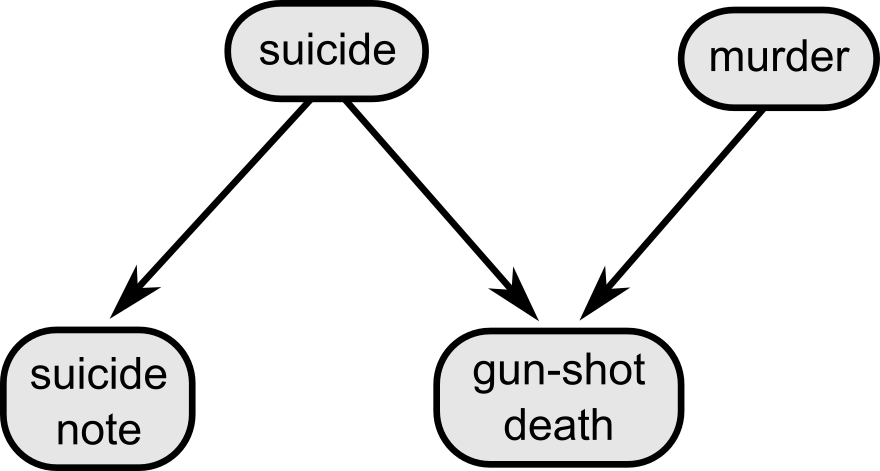
\includegraphics[scale=0.6]{suicide-note-en.png}}}
\end{equation}

At the sub-propositional level, every proposition may be represented as an entity-relation graph, where each node is a \textbf{concept atom}:
\begin{equation}
\vcenter{\hbox{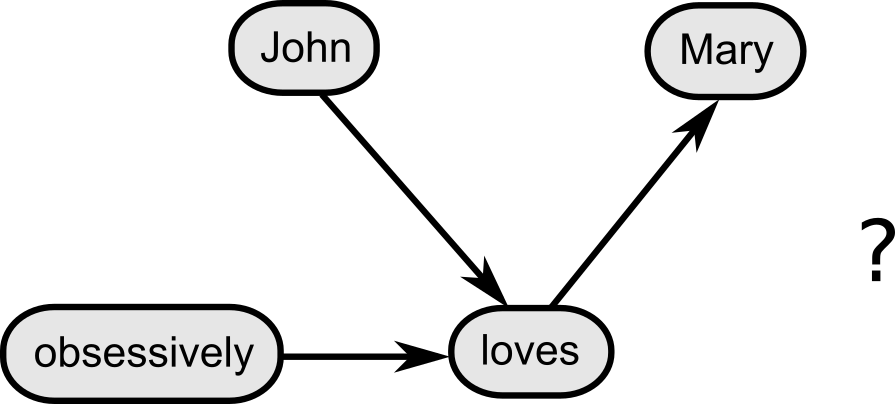
\includegraphics[scale=0.6]{John-loves-Mary-obsessively.png}}}
\end{equation}
but we are still unsure about the exact construction mechanism of sub-propostional graphs.

\subsection{Episodic memory}

Episodic memory = an even-bigger graph?

\section{NN acting on graphs}

\subsection{CNN}

With this analogy:
\begin{equation}
\mbox{CNN for vision} \quad \Longleftrightarrow \quad \mbox{CNN for graphs}
\end{equation}
a new breed of algorithms have been developed, eg: \citep{Niepert2016} \citep{Defferrard2016} \cite{Kipf2016}.  For a nice introduction see the blog entry: \url{https://tkipf.github.io/graph-convolutional-networks/}.

As explained in \citep{Niepert2016}, a CNN works as if a ``receptive field'' moves over an image:
\begin{equation}
\vcenter{\hbox{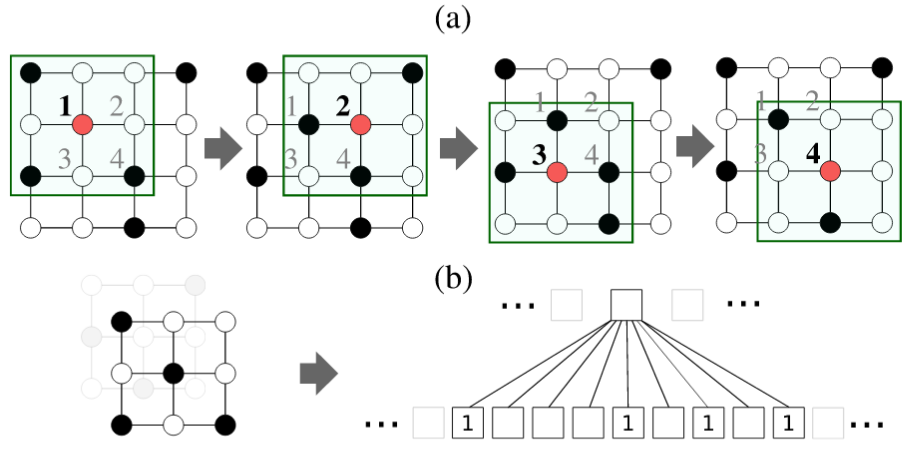
\includegraphics[scale=0.4]{CNN-explained.png}}}
\end{equation}
and the idea is to let a similar receptive field \uline{traverse a graph}.

\section{Cartesian closure}

\ifdefined\chinchin
举例来说,「吃了污糟的食物会肚痛」是一个句子,它经由 $\Eye$ 进入 mental state $\vect{x}$ ,变成 proposition。 但我们希望这逻辑命题变成 $\KB$ 的一部分。With
\else
For example, ``eating dirty food causes stomach pains'' is an NL sentence, it enters from $\Eye$ into the mental state $\vect{x}$, as a \textbf{proposition}.  But we want $\vect{x}$ to become part of $\KB$.  With
\fi
\begin{equation}
\vect{x}' = \vect{f}(\vect{x})
\end{equation}
where \\
\tab $\vect{f} = \KB = \NN$ \\
\tab $\vect{x} = $ state

An individual logic rule is a \uline{restriction} of $\vect{f}$ to a specific input.

$\vect{f} \equiv \KB$ is the \uline{sum of restrictions}:
\begin{equation}
\KB = \bigcup \vect{f}_i
\end{equation}
Or roughly speaking, $\vect{f}$ is the sum total of objects like $\vect{x}$:
\begin{equation}
\vect{f} = \bigcup \vect{x}_i
\end{equation}

However, the problem is that the structure of $\vect{f}$ (as the neural network $\NN$) is too complicated to be expressed as a sum of restricted functions.  This remains an unsolved problem.

\section*{Acknowledgements}

Thanks to Jonathan Yan for suggesting to use CNN for graphs and showed me the relevant papers.

\bibliographystyle{unsrtnat} % or number or aaai ...
\bibliography{AGI-book}

\end{document}
